\ifx\wholebook\relax \else

\documentclass[b5paper]{ctexart}
\usepackage[nomarginpar
  %, margin=.5in
]{geometry}

\addtolength{\oddsidemargin}{-0.05in}
\addtolength{\evensidemargin}{-0.05in}
\addtolength{\textwidth}{0.1in}

\usepackage[cn]{../prelude}

\setcounter{page}{1}

\begin{document}

\title{无理数}

\author{刘新宇
\thanks{{\bfseries 刘新宇} \newline
  Email: liuxinyu99@hotmail.com \newline}
  }

\maketitle
\fi

\markboth{无理数}{数的旅程}

\ifx\wholebook\relax
\chapter{无理数}
\fi

\epigraph{数学是上帝用来书写宇宙的文字}{伽利略}

公元前240年的夏至中午,这一天是一年中日照最长的一日,大约是现代历法的6月21日附近。埃及亚历山大港图书馆馆长埃拉托斯特尼(公元前276年~194年)正和一位来自赛印城的商人交谈。赛印(Syene)位于今天埃及南部的阿斯旺,是北回归线上的一个城市。“我的老家是世上最干最热的地方。”商人说道:“我们打了很深的井汲水,每年的这个时候,阳光能射到井底呢。”听到这句话时埃拉托斯特尼注意到了到广场上纪念碑的影子。为什么会这样呢?除非大地不是平坦的,而是球形。他询问哪个商人:“从赛印城到亚历山大有多远的路程?”“有5000斯塔蒂亚。”斯塔蒂亚(Stadia)是古希腊的长度单位,约和158米。埃拉托色特尼测量了立在地上的杆子和影子的长度,发现杆子的长度大约是影子长度的8倍。他于是按照\cref{fig:eratosthenes-earth}进行了计算。

\begin{figure}[htbp]
 \centering
 \subcaptionbox{太阳在夏至直射北回归线上的赛印城\label{fig:eratosthenes-earth}}{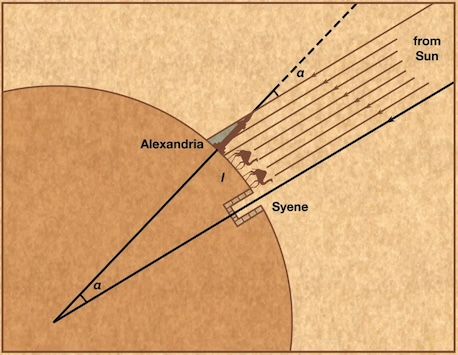
\includegraphics[scale=0.35]{img/eratosthenes-earth}}
 \subcaptionbox{太阳照射亚历山大的角度为$\alpha$\label{fig:atan8}}{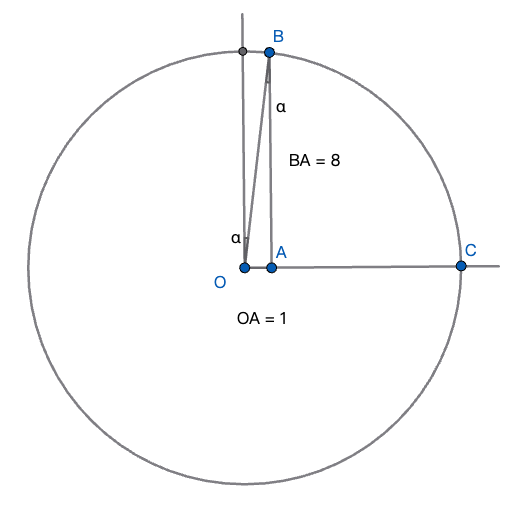
\includegraphics[scale=0.32]{img/atan8}}
 \caption{埃拉托斯特尼测量地球}
\end{figure}

夏至正午时刻,太阳直射北回归线,因此阳光可以射入赛印城的井底。埃拉托色特尼可以通过\cref{fig:atan8}找出阳光照射亚历山大港的角度。
%% 这相当于今天高中数学中的反正切$\arctan(\frac{1}{8})$。
但当时古巴比伦的角度单位还没有传入古希腊,按照埃拉托斯特尼的说法,这个角度是圆的50分之一,合$7.2\degree$。太阳光是平行光。如果大地是球形的,那么赛印城和亚历山大到球心的张角,是太阳入射角的同位角(\cref{fig:eratosthenes-earth}中标有$\alpha$的两个角),也是圆的50分之一。所以赛印城到亚历山大之间的距离就是地球周长的50分之一。这样算来,地球的周长就是$50 \times 5000 = 250000$斯塔提雅,约合$250 \times 158 = 39500 \approx 4$万千米。而今天人们通过人造卫星测得地球赤道长度为40075千米。埃拉托色特尼的著作没有流传到今天,我们从古希腊数学家帕普斯等人的记述中了解到他的具体测量方法。埃拉托色特尼约在公元前235年起任亚历山大图书馆馆长,他对地球的测量发生在这一时期\cite{Walkup2005}。赛印城到亚历山大的距离是一个关键,5000斯塔蒂亚无疑是一个大致数字。埃拉托斯特尼可能通过多种途径核证该距离,包括询问往来的商人以及测量地图。赛印城和亚历山大港都是尼罗河沿岸城市,尼罗河有规律的每年泛滥,埃及人因此每年在泛滥后重新丈量尼罗河沿线的土地并更新地图。此外,古希腊的斯塔蒂亚到底有多长学者们也有不同的观点。无论如何,埃拉托色特尼在2000年前的伟大推理和计算无疑是惊人的。

\begin{figure}[htbp]
 \centering
 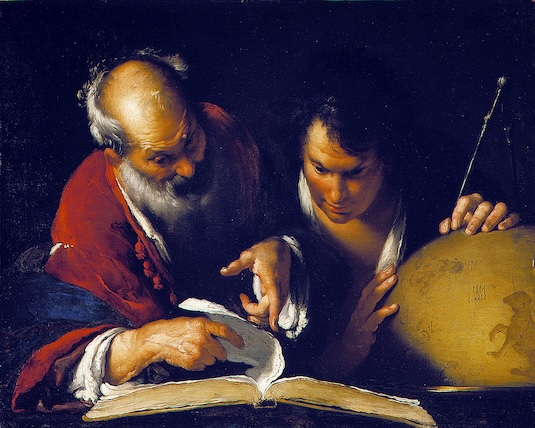
\includegraphics[scale=0.35]{img/eratosthenes}
 % https://commons.wikimedia.org/wiki/File:Eratosthenes_Teaching_in_Alexandria_(Bernardo_Strozzi,_Montreal).jpg
 \caption{贝尔纳多·斯特罗齐于1635年创作的油画:在亚历山大教学的埃拉托色特尼}
 \label{fig:eratosthenes}
\end{figure}

马其顿国王亚历山大大帝征服埃及后,兴建了以他命名的城市亚历山大港,成为了希腊化时代的文化和学术中心。埃拉托色特尼测量地球的壮举通常被认为是体现古希腊几何学力量的典范。古希腊并没有位值制计数系统(见第1章),但却发展出了严密的推理和几何学传统。正是在把数和几何学结合后,古希腊人\underdot{发现}了无理数,使得数的大家庭又得到了一次扩充。

\section{万物皆数}
音乐与数似乎毫无关联,但毕达哥拉斯却发现了它们背后竟有奇妙的规律。他从中得到启发并大胆推测“万物皆数”(All is number),认为世间万物都可以用数或数的比例来理解。毕达哥拉斯可以说是用数探索世间万物的第一人。他出生于希腊的萨摩斯(Samos)岛,年轻时他曾去米利都(Miletus)向古希腊哲学的奠基人泰勒斯(Thales)学习。在泰勒斯的建议下,毕达哥拉斯于公元535年前往埃及学习数学。公元前525年,波斯帝国征服了埃及,他被俘并随军向东到达了巴比伦。毕达哥拉斯得以向巴比伦人学习数学和天文知识。或许后来他还到达了更远的印度。不论到了哪里,毕达哥拉斯都不断向有学问的人请教,丰富自己的见解。重要的是,他不仅刻苦学习,而且更善于思考。在经过兼收并蓄、汲取各家之长后,毕达哥拉斯形成并完善了自己的思想\cite{HanXueTao16}。

经历了漫长的在外游历后,年近半百的毕达哥拉斯返回了故乡萨默斯并开始讲学。公元前520年左右,也许为了摆脱当地的暴政,毕达哥拉斯移居到了意大利南部的克罗顿(Croton)发展。在那里他赢得了人们的信任与景仰并形成了自己的学派。毕达哥拉斯的弟子中还有女性,学派把主要精力都用来研究天文、几何、数论、音乐这四门学科。它们被称为四术(quadrivium),影响了欧洲教育两千多年\cite{StepanovRose15}。四术体现了毕达哥拉斯万物皆数的哲学思想:星体的运动与几何对应,而几何又以数为基础,数字还可以衍生出音乐(见第3章)。关于毕达哥拉斯去世有多种说法。他领导的学派具有很高的声誉和政治影响,引起了敌对派的忌恨。约公元前497年,学派在克罗顿的活动场所遭到破坏。有人认为毕达哥拉斯被暴徒杀害,也有人说他逃到梅塔蓬图姆(Metapontum)并度过余生\cite{MKlein1972}。

\index{形数(figurate number)}
毕达哥拉斯学派研究数字,认为数与数、数与自然之间存在着神秘关系。这开启了数学的重要分支——数论。学派对正整数进行了分类,定义了奇数、偶数、素数、合数等。他们通过在地上摆小石子来研究数字,英文的计算calculus一词就是从希腊文“石子”衍生出的\cite{HanXueTao16}。当把石子按照某种几何图形摆放时,就得到了形数(figurate number)。

\begin{figure}[htbp]
%\begin{wrapfigure}{R}{0.4\textwidth}
\centering
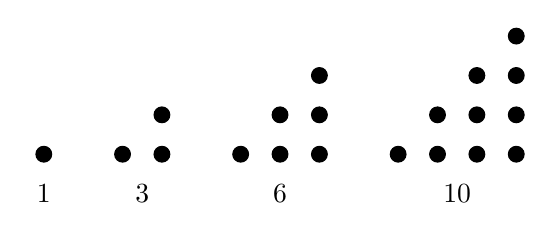
\begin{tikzpicture}[scale=0.5]
\filldraw (0, 0) circle (0.2);
\draw (0, -1) node{1};
\filldraw (2, 0) circle (0.2)
          (3, 0) circle (0.2)   (3, 1) circle (0.2);
\draw (2.5, -1) node{3};
\filldraw (5, 0) circle (0.2)
          (6, 0) circle (0.2)   (6, 1) circle (0.2)
          (7, 0) circle (0.2)   (7, 1) circle (0.2)   (7, 2) circle (0.2);
\draw (6, -1) node{6};
\filldraw (9, 0) circle (0.2)
          (10, 0) circle (0.2)    (10, 1) circle (0.2)
          (11, 0) circle (0.2)    (11, 1) circle (0.2)    (11, 2) circle (0.2)
          (12, 0) circle (0.2)    (12, 1) circle (0.2)    (12, 2) circle (0.2)    (12, 3) circle (0.2);
\draw (10.5, -1) node{10};
\end{tikzpicture}
\caption{三角形数(triangular number)}
\label{fig:triangular-num}
%\end{wrapfigure}
\end{figure}

\begin{figure}[htbp]
%\begin{wrapfigure}{R}{0.4\textwidth}
\centering
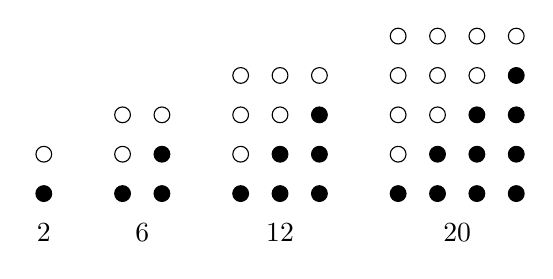
\begin{tikzpicture}[scale=0.5]
\draw (0, 1) circle (0.2);
\filldraw (0, 0) circle (0.2);
\draw (0, -1) node{2};

\draw (2, 1) circle (0.2)   (2, 2) circle (0.2)
      (3, 2) circle (0.2);
\filldraw (2, 0) circle (0.2)
          (3, 0) circle (0.2)   (3, 1) circle (0.2);
\draw (2.5, -1) node{6};

\draw (5, 1) circle (0.2)   (5, 2) circle (0.2)   (5, 3) circle (0.2)
      (6, 2) circle (0.2)   (6, 3) circle (0.2)
      (7, 3) circle (0.2);
\filldraw (5, 0) circle (0.2)
          (6, 0) circle (0.2)   (6, 1) circle (0.2)
          (7, 0) circle (0.2)   (7, 1) circle (0.2)   (7, 2) circle (0.2);
\draw (6, -1) node{12};

\draw (9, 1) circle (0.2)   (9, 2) circle (0.2)   (9, 3) circle (0.2)   (9, 4) circle (0.2)
      (10, 2) circle (0.2)   (10, 3) circle (0.2)   (10, 4) circle (0.2)
      (11, 3) circle (0.2)   (11, 4) circle (0.2)
      (12, 4) circle (0.2);
\filldraw (9, 0) circle (0.2)
          (10, 0) circle (0.2)    (10, 1) circle (0.2)
          (11, 0) circle (0.2)    (11, 1) circle (0.2)    (11, 2) circle (0.2)
          (12, 0) circle (0.2)    (12, 1) circle (0.2)    (12, 2) circle (0.2)    (12, 3) circle (0.2);
\draw (10.5, -1) node{20};
\end{tikzpicture}
\caption{长方形数(oblong number)}
\label{fig:oblong-num}
%\end{wrapfigure}
\end{figure}

\cref{fig:triangular-num}和\cref{fig:oblong-num}分别是三角形数和长方形数。容易看出,每个长方形数都对应三角形数的二倍,而三角形数又是前$n$个正整数之和,这样就得到了正整数累加的求和公式:

\[
1 + 2 + 3 + ... + n = \frac{1}{2}n(n+1)
\]

毕达哥拉斯学派还观察到,所有的奇数可以表示成折尺形(或称为“磬折形”)\footnote{gnomon这个字在巴比伦人的原意可能是指日晷上的直杆,用它的阴影来指示时刻。在毕达哥拉斯时代,gnomon指木匠用的方尺。它还表示从正方形的一角切掉一个小正方形后剩余的图形。以后欧几里得又把正方形扩展到平行四边形\citepage[26页]{MKlein1972}。},如\cref{fig:gnomon-num},而前$n$个折尺形可以拼成一个正方形,如\cref{fig:square-num}。这样他们就发现了前$n$个正奇数的求和公式:

\[
1 + 3 + 5 + ... + (2n - 1) = n^2
\]

\begin{figure}[htbp]
%\begin{wrapfigure}{R}{0.4\textwidth}
\centering
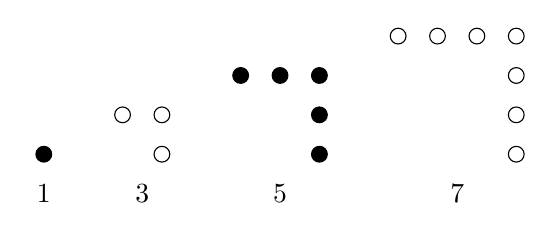
\begin{tikzpicture}[scale=0.5]
\filldraw (0, 0) circle (0.2);
\draw (0, -1) node{1};

\draw (2, 1) circle (0.2)
      (3, 0) circle (0.2)   (3, 1) circle (0.2);
\draw (2.5, -1) node{3};

\filldraw (5, 2) circle (0.2)   (6, 2) circle (0.2)   (7, 2) circle (0.2)
          (7, 0) circle (0.2)   (7, 1) circle (0.2);
\draw (6, -1) node{5};

\draw (9, 3) circle (0.2)   (10, 3) circle (0.2)   (11, 3) circle (0.2)   (12, 3) circle (0.2)
      (12, 0) circle (0.2)    (12, 1) circle (0.2)    (12, 2) circle (0.2);
\draw (10.5, -1) node{7};
\end{tikzpicture}
\caption{折尺形数(gnomon number)}
\label{fig:gnomon-num}
%\end{wrapfigure}
\end{figure}

\begin{figure}[htbp]
%\begin{wrapfigure}{R}{0.4\textwidth}
\centering
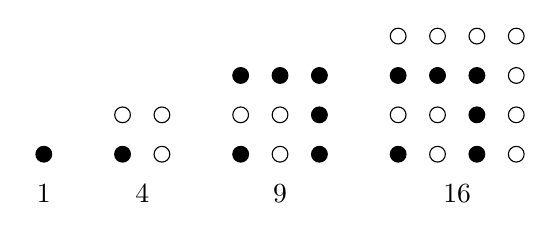
\begin{tikzpicture}[scale=0.5]
\filldraw (0, 0) circle (0.2);
\draw (0, -1) node{1};

\filldraw (2, 0) circle (0.2);
\draw (2, 1) circle (0.2)
      (3, 0) circle (0.2)   (3, 1) circle (0.2);
\draw (2.5, -1) node{4};

\filldraw (5, 0) circle (0.2);
\draw (5, 1) circle (0.2)
      (6, 0) circle (0.2)   (6, 1) circle (0.2);
\filldraw (5, 2) circle (0.2)   (6, 2) circle (0.2)   (7, 2) circle (0.2)
          (7, 0) circle (0.2)   (7, 1) circle (0.2);
\draw (6, -1) node{9};

\filldraw (9, 0) circle (0.2);
\draw (9, 1) circle (0.2)
      (10, 0) circle (0.2)   (10, 1) circle (0.2);
\filldraw (9, 2) circle (0.2)   (10, 2) circle (0.2)   (11, 2) circle (0.2)
          (11, 0) circle (0.2)   (11, 1) circle (0.2);
\draw (9, 3) circle (0.2)   (10, 3) circle (0.2)   (11, 3) circle (0.2)   (12, 3) circle (0.2)
      (12, 0) circle (0.2)    (12, 1) circle (0.2)    (12, 2) circle (0.2);
\draw (10.5, -1) node{16};
\end{tikzpicture}
\caption{正方形数(square number)与折尺形数的关系}
\label{fig:square-num}
%\end{wrapfigure}
\end{figure}

就这样,毕达哥拉斯学派把几何形状也建立在了数的基础上。他们热衷与用数去解释更多的现象,并相信宇宙的本质就在于“数的和谐”,由此出发,毕达哥拉斯学派试图发展一套以数字为基础的理论,使得几何学可以建立在该理论之上。

\section{勾股定理}
毕达哥拉斯学派最著名的发现当属勾股定理,在西方叫做“毕达哥拉斯定理”。据说毕达哥拉斯对他发现的这个定理及其证明极为高兴,为此献祭了一百头公牛庆贺。但脍炙人口的传说故事往往不真实。毕达哥拉斯学派对团体成员有着极为严格的戒律,任何人的研究发现都归学派所有并必须保密。我们所知的以“毕达哥拉斯”命名的成果大都来自学派内的佚名作者。勾股定理并非孤立成果,各个文明都各自独立发现了它。如第3章中的\cref{fig:babylonian-yale}所示,这块古巴比伦泥板的时间大约是公元前1900年~1600年,此外人们还发现了刻有勾股数表的泥板。古埃及的测量员绳子作为软尺(称为拉绳人)。相传他们在绳上打结,把全长分成长度为3比4比5的三段,然后用来形成直角三角形。但这个说法没有文献证实\citepage[16页]{MKlein1972}。古印度数学家包德哈亚那(Baudhayana,生活在公元前800年到公元前400年间)的著作《绳法经》(Śulba Sutra)也提到了这个定理。在古代中国,成书于公元前一世纪的《周髀算经》中载有西周时代(约公元前11世纪)周公和商高的一段对话,其中提到“勾三、股四、弦五”\footnote{商高说:“……故折矩,勾广三,股修四,经隅五。”},故在中国称之为“勾股定理”。《九章算术》的注解中载有三国时代的赵爽和魏晋时刘徽给出的勾股定理证明\footnote{对赵爽和刘徽给出的究竟是严格意义的证明还是某种程度的解释历来有不同观点。}。

这一定理自提出以来,吸引了无数聪明的头脑对它进行证明。如今在中学数学课堂上就至少有“赵爽弦图”(见\cref{fig:cms-zhaoshuang}),传说中的“毕达哥拉斯证法”(见\cref{fig:pythagoras-pww})和《原本》证法。在4000年的时间里,诞生了超过300多种不同的证明,包括意大利文艺复兴时期的全才达芬奇(见\cref{fig:davinci})和美国总统加菲尔德。

\begin{figure}[htbp]
 \centering
 \subcaptionbox{中国数学会会徽\label{fig:cms-logo}}{
\includegraphics[scale=0.5]{img/cms}} \quad
 \subcaptionbox{赵爽弦图\label{fig:zhaoshuang}}{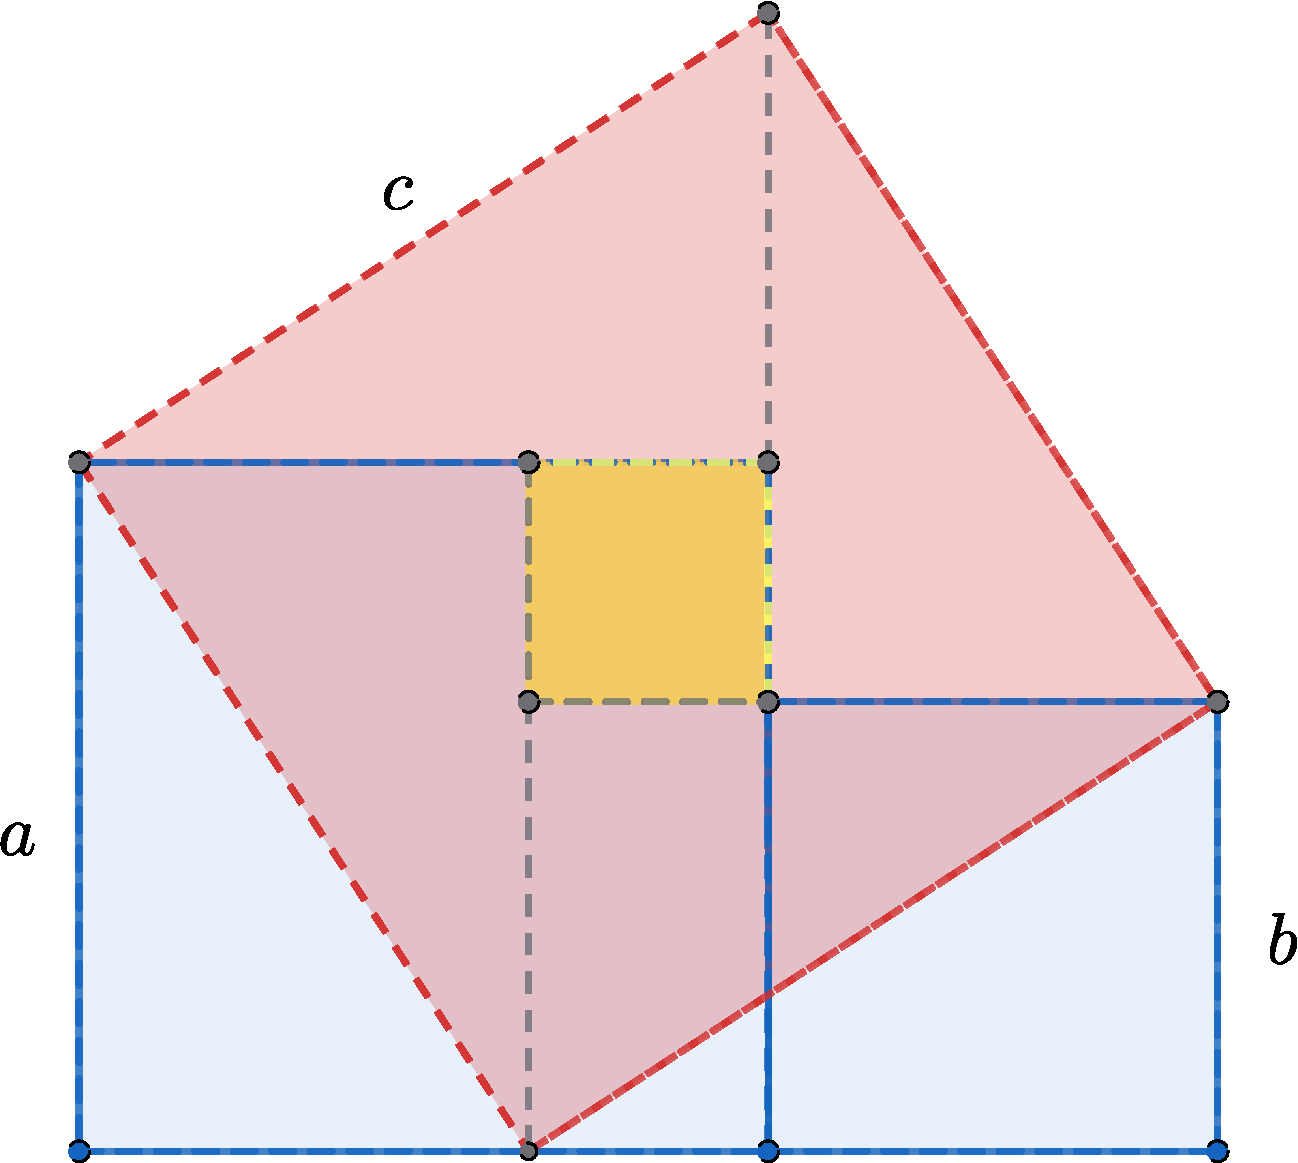
\includegraphics[scale=0.2]{img/zhaoshuang}}
 \caption{赵爽弦图成为了2002年在北京召开的国际数学家大会和中国数学会的会徽。\label{fig:cms-zhaoshuang}}
\end{figure}

\begin{figure}[htbp]
 \centering
 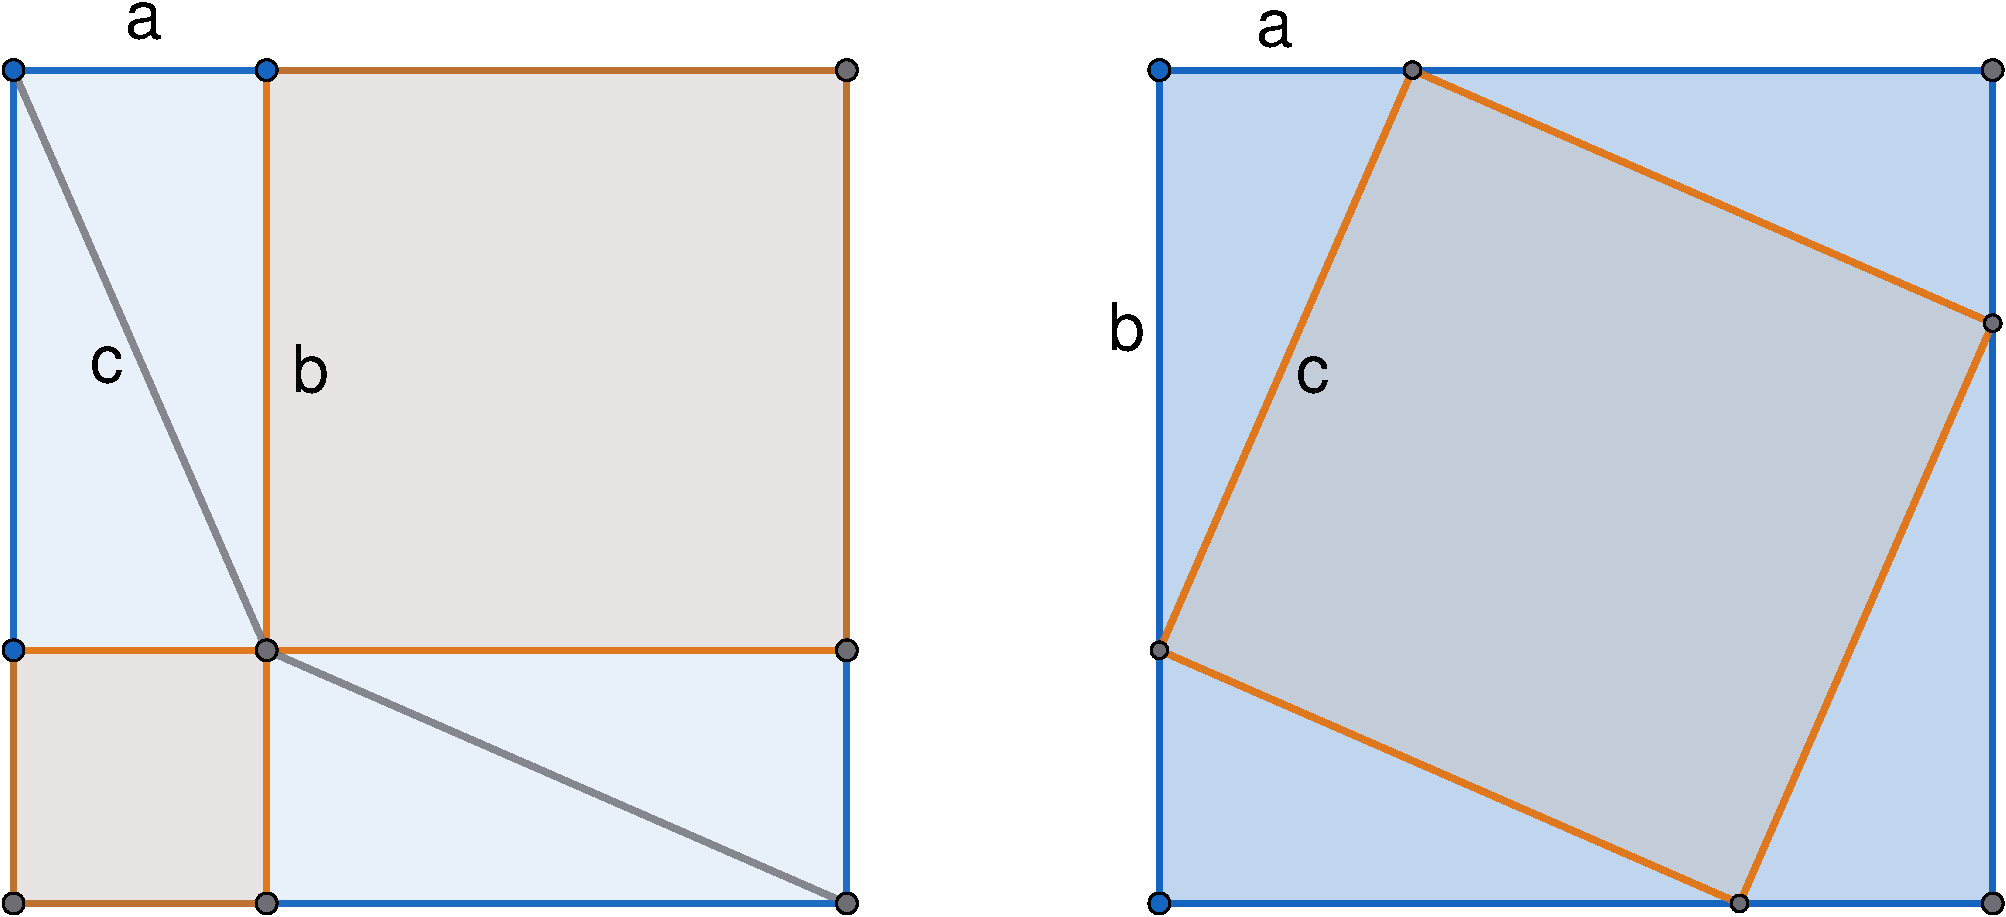
\includegraphics[scale=0.3]{img/pythagoras-pww}
 \caption{传说中的毕达哥拉斯证法\label{fig:pythagoras-pww}}
\end{figure}

达芬奇的方法把原直角三角形复制两份:一份上下颠倒拼到上方,一份平移拼到斜边组成的正方形下方。此时把\cref{fig:davinci}中的“T”形点划线上方的四边形左右镜像翻转,就拼出一个和下方全等的六边形。它们的面积相等,因此各自减去两个原直角三角形的面积后仍相等,即$a^2 + b^2 = c^2$。\cref{qn:pythagoras-thm-garfield}要求解释美国总统加菲尔德的证明方法。

\begin{figure}[htbp]
 \centering
 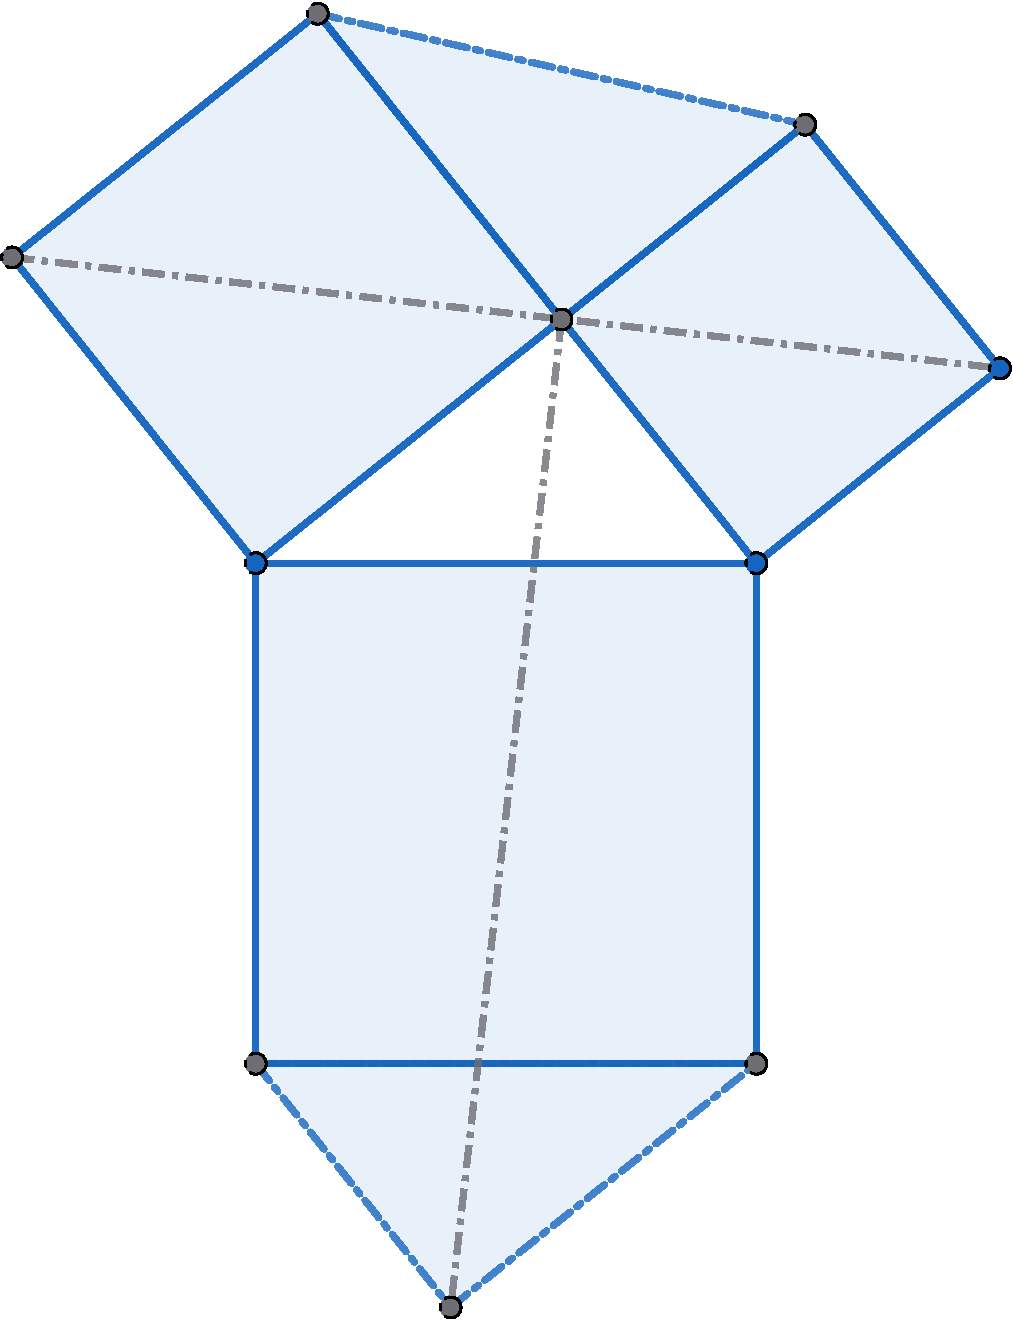
\includegraphics[scale=0.3]{img/davinci}
 \caption{列昂纳多·达·芬奇证法\label{fig:davinci}}
\end{figure}

勾股定理具有非凡的意义,犹如发源的清泉,流淌出了三条壮阔的大河\cite{Stillwell-2010}:1)数论,通过寻找哪些数构成勾股数(也叫做毕达哥拉斯三元组),古希腊人开启了数学皇冠上的明珠——数论的研究。2)几何,勾股定理本身就是一条定量的几何定理。3)无穷,把勾股定理和欧几里得算法结合,古希腊人被无穷次的递归困扰,直接导致了无理数的发现。

\section{数论}
并非任意两个平方数的和一定是平方数,例如$3^2 + 5^2 = 34$不是任何正整数的平方。我们把满足勾股定理的三个正整数$(a, b, c)$叫做勾股数或毕达哥拉斯三元组\footnote{Pythagoras triple}。各个文明都发现了常见的勾股数如$3^2 + 4^2 = 5^2$,$5^2 + 12^2 = 13^2$。古巴比伦的石板上刻有长长的勾股数表。那么究竟怎样找到勾股数?勾股数是有限多还是无限多?这个问题是欧几里得彻底解决的。欧几里得指出,如果$a^2 + b^2 = c^2$成立,那么这组勾股数的倍数也是勾股数,因为:

\begin{align*}
(ka)^2 + (kb)^2 &= k^2(a^2 + b^2) & \text{分配律} \\
  &= k^2c^2 & \text{由}a^2 + b^2 = c^2 \\
  &= (kc)^2
\end{align*}

反过来,如果$a, b$含有公因子$k \ne 1$,则$k$一定也是$c$的因子。同理,如果$b, c$含有公因子$k$,则由于$a^2 = c^2 - b^2$,所以$k$一定也是$a$的因子。本质上我们只需要寻找彼此互素的$a, b, c$(公因子只有1,或$(a, b) = (b, c) = 1$,见\ref{sec:gcd-minus}节),然后乘上倍数就得到更多的勾股数。例如勾股数(12, 16, 20)都是偶数,显然含有公因子2。分别除以2就得到更“简单”的勾股数(6, 8, 10)。继续除以2得到(3, 4, 5)。此时3、4、5彼此互素,已经不能再化简了。我们不妨称这样的勾股数为“最简勾股数”。由于$a$和$a^2$的奇偶相同:奇数的平方还是奇数,偶数的平方还是偶数。如果$a, b$一奇一偶,则$c$一定是奇数。欧几里得进一步排除了$a, b$都是奇数的情况,因为:

\begin{align*}
a^2 + b^2 &= (2m + 1)^2 + (2n + 1)^2 & \text{把}a, b\text{写成奇数形式} \\
  &= 4m^2 + 4m + 1 + 4n^2 + 4n + 1 & \text{分别用完全平方公式展开} \\
  &= 4(m^2 + m + n^2 + n) + 2 = 4k + 2 & \text{令整数} k = m^2 + m + n^2 + n
\end{align*}

这个值除以4余2。但是不管$c$是奇数还是偶数,$c^2$除以4都不可能余2。因为:偶数$(2k)^2 = 4k^2$被4整除,而奇数$(2k + 1)^2 = 4(k^2 + k) + 1$除以4余1。因此$a$和$b$不可能都是奇数,只能是一奇一偶。我们可以任选一个(比如第一个)为偶数,另一个是奇数。这样问题就化简为寻找第一个数为偶数,彼此互素的勾股数。它的答案赫然出现在《几何原本》卷十中的引理1\footnote{《几何原本》中使用正方形代表平方数,并用语言描述做法,见\citepage[330页]{Elements}。这里使用代数符号方便理解。}。

\begin{lemma}[欧几里得《几何原本》卷十,引理1]
方程$x^2 + y^2 = z^2$其中$x, y, z$彼此互素,且$x$是偶数的\underdot{所有}正整数解,可表示为:
\be
\begin{cases}
x = 2mn \\
y = m^2 - n^2 \\
z = m^2 + n^2
\end{cases}
\ee
其中$m > n$,是奇偶不同且互素的任意正整数。
\end{lemma}

注意“所有”二字,这意味着不存在其它最简勾股数能逃出欧几里得的解。换言之,这是\underdot{充分必要}条件。我们接下来证明这一优美的结论。

\begin{proof}
首先正向证明充分性:

\begin{align*}
x^2 + y^2 &= (2mn)^2 + (m^2 - n^2)^2 & \text{代入} \\
  &= 4m^2n^2 + m^4 + n^4 - 2m^2n^2 & \text{完全平方公式展开} \\
  &= m^4 + n^4 + 2m^2n^2 = (m^2 + n^2)^2 &\text{反向用完全平方公式} \\
  &= z^2 &\text{代入}z
\end{align*}

接下来反向证明必要性。把$x^2 + y^2 = z^2$移项后用平方差公式:
\begin{align}
x^2 &= z^2 - y^2 = (z + y)(z - y) &\text{平方差公式} \label{eq:x-as-z-pm-y} \\
(\frac{x}{2})^2 &= (\frac{z + y}{2}) (\frac{z - y}{2}) &\text{左右同除以4}
\end{align}

$x$是偶数,$y, z$都是奇数,故$z \pm y$都是偶数。因此左边的$\frac{x}{2}$,右边的$\frac{z \pm y}{2}$都是正整数。进一步,由于$z, y$互素,所以$\frac{z + y}{2}$和$\frac{z - y}{2}$也互素(见\cref{qn:coprime-of-half-a-pm-b})。如果两个互素的数的乘积是一个平方数,则它们也都是平方数(见\cref{qn:coprime-product-as-square})。因此:

\begin{align*}
\frac{z+y}{2} &= m^2 \\
\frac{z-y}{2} &= n^2
\end{align*}

其中正整数$m > n$。两式相加消去$y$求得$z = m^2 + n^2$,两式相减消去$z$求得$y = m^2 - n^2$。代入\cref{eq:x-as-z-pm-y}得:$x^2 = 2m^2 2n^2$,故$x = 2mn$。
\end{proof}

例如取$m = 2, n = 1$就得到(3, 4, 5),取$m = 3, n = 2$就得到(12, 5, 13)。而所有勾股数的就可以表示为:

\be
x = 2mnr, \quad y = r(m^2 - n^2), \quad z = r(m^2 + n^2)
\ee

其中$r$是任意正整数。

\begin{figure}[htbp]
 \centering
 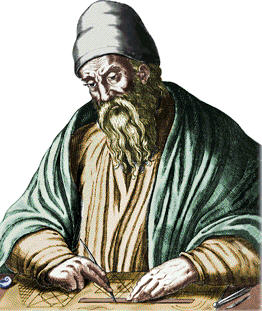
\includegraphics[scale=0.6]{img/Euclid}
 \caption{欧几里得,约公元前300年前后}
 \label{fig:Euclid}
\end{figure}

\begin{mdframed}

\index{欧几里得}
欧几里得(Euclid)是古希腊数学家,以其所著的《几何原本》闻名于世。对于他的生平,现在知道的很少。柏拉图学派晚期的导师普罗克洛斯(Proclus)在《几何学发展概要》中记述了这样的趣事:当时的埃及国王,亚历山大的托勒密一世有一次问欧几里得,学习几何学又没有什么捷径可走。欧几里得回答到:“在几何里,没有专为国王铺设的大道。\footnote{也译为“几何无王者之道”}”(There is no royal road to geometry),学习没有捷径成为了千古传颂的箴言。斯托比亚斯(Stobaeus)记述另一则故事说。一个学生刚开始学习第一个命题,就问欧几里得学习几何后将得到什么。欧几里得说:“给他三个钱币,因为他想在学习中获取实利。”由此可知欧几里得主张学习必须循序渐进、刻苦钻研、不赞成投机取巧的作风,也反对狭隘的实用观点\cite{Elements}。

欧几里得的《几何原本》是一部划时代的著作。其伟大的历史意义在于它是用公理建立起演绎体系的最早典范。过去所积累下来的数学知识是零碎的、片断的,可以比作木石砖瓦。只有借助于逻辑方法,把这些知识组织起来,加以分类比较,解释彼此间的内在联系,整理在一个严密的系统之中,才能建成巍峨的大厦。《几何原本》完成了这一艰巨的任务,它对整个数学的发展产生了深远的影响。

《几何原本》的英文译作The thirteen books of Euclid's elements,直译成中文是欧几里得原本十三卷,简称《原本》(英文简称Elements)。这十三卷包含几何、恒等式、比例论、数论、无理量、穷竭法、正多面体等内容,是古希腊数学的集大成者。明代末年,《原本》前六卷传入中国,学者徐光启和传教士利玛窦与1607年合作将其翻译成中文。可能是因为前六卷集中于几何学(第十卷才包含数论),徐光启将其命名为《几何原本》。其中译定的一些重要术语沿用至今。遗憾的是,利玛窦的去世和明清之际的剧变中断了后七卷的翻译工作。直到250年后的1857年,中国数学家李善兰和英国传教士伟烈亚力才将完整的《几何原本》译出。他们以英译本为底本,译出了后九卷,包括被认为是后人添加的第14,15卷。李善兰曾在曾国藩军中效力,他把译稿交给曾国藩说,松江刻本已经毁于战乱了,如果不再出版,这样的绝学就会失传(“此算学家不可少之书,失今不刻,行复绝矣。”)。曾国藩嘱托李善兰把前六卷重新订正,汇集在一起。同治四年(1865年)十月,曾国藩为此书作序,并主持重刻出版。这推动了《几何原本》在近代中国的传播和影响。考虑到这十三卷的内容不仅包含几何,今天在部编版中小学数学教材中,已经统一使用《原本》这个译法。我们也推荐读者朋友们使用《原本》或者《欧几里得原本》这样的叫法。
%% https://www.zhonghuashu.com/wiki/%E5%B9%BE%E4%BD%95%E5%8E%9F%E6%9C%AC/%E5%BA%8F

两千多年来,这部著作在几何教学中一直占据统治地位,在二十世纪初依然用于数学课的基本教材。包括我国在内的许多国家仍将其作为中学的必修科目(现在中学的几何课本是按照法国数学家勒让德《原本》改写本思路编写的),并作为训练逻辑推理的最有力教育手段\cite{HanXueTao16}。
\end{mdframed}

尽管彻底解决了$x^2 + y^2 = z^2$的所有整数解问题,但$x^3 + y^3 = z^3$,$x^4 + y^4 = z^4$,或者更一般的$x^n + y^n = z^n$(其中整数$n \geq 3$)却难住了古人。似乎除了$x = y = z = 0$再也找不出任何整数解了。我们要等到1800年后的十七世纪,青年“业余”数学家费马才在$n = 4$上获得突破(见第6章)。勾股定理的整数解问题展示了数论这一数学分支的典型问题:研究数,特别是整数的性质。在很长一段时间,这门学科被称为“算术”(arithmetic),例如古希腊数学家丢番图的名著《丢番图算术》,德国数学家高斯的化时代著作《算术研究》都是数论方面的经典。奇偶性、素数、整除、公因子,余数等概念是这门学科的基础概念。在“长方形数”的探索中,古希腊人发现某些数可以表示成长方形,如$12 = 3 \times 4$可以用三行四列的小石子摆出。这样就引出了因数的概念,长方形数的边长就是其因子。并且因子可能有多个,例如$12 = 3 \times 4 = 2 \times 6$,所以2、3、4、6都是12的因子。但是有些数却无法表示成长方形数,例如5,只能摆成一行五个石子或一列五个石子\footnote{显然古希腊人在这里区分了线段和矩形,他们并不认可$1 \times 5$或$5 \times 1$是一个长方形数。}。这种数形结合的方法引出了素数的概念。素数$p$只能被1和$p$整除,是构成其它数的砖石。前几个素数是2、3、5、7、11……这样的探索自然引出了有趣的问题:1)作为构成其它数的砖石,素数有多少个?是有限多还是无限多?2)素数的出现有何规律?有没有产生素数的公式和方法?其中第一个问题又是由欧几里得解决的,而埃拉托斯特尼在第二个问题上迈出了关键的第一步。

自从芝诺悖论提出后,古希腊人就试图避免无穷这个概念。亚里士多德认为所有芝诺悖论中的问题都源自无穷,他提出了一个影响至今的区分:潜无穷和实无穷\footnote{英文分别是potential infinity和actual infinity}。所谓潜无穷或潜无限,是指无限在永远延伸着,是一种变化的、不断产生出来概念。它永远在构造中,永远完成不了,是潜在的,而不是实在的。自然数就是一种潜无穷,对于任何一个自然数$n$,我们都可以找到它的后继$n + 1$,也就是一个更大的自然数。欧几里得几何中的直线也是一种潜无穷,我们可以按需延伸直线。所谓实无穷是指把无限的整体本身作为一个实在的单位,是已经构造出来的东西。也就是把无限对象看作可完成的过程或无穷整体。在做了这种区分后,亚里士多德承认存在潜无穷,但是拒绝承认实无穷的概念。他对实无穷的排斥深刻而长远地影响了日后数学的发展\cite{HanXueTao16}。亚里士多德代表了当时古希腊的哲学观点,关于潜无穷和实无穷的概念区分以及争论一直影响至今。纵观《原本》全书,欧几里得从未在其中使用“无穷”或者“无限”一词。尽管如此他还是成功证明了素数有无限多个,并且这一证明被人们认为是历史上最优美的证明证明之一。

\begin{theorem}[欧几里得《原本》第九卷,命题20]
预先给定任意多的素数,则有比它们更多的素数。
\end{theorem}

欧几里得在叙述这个命题时,小心谨慎地避免使用无穷这样的说法。“预先给定……总有更多的……”这种处理经常出现在《原本》中。我们今天往往直接说“存在无穷多的素数”。欧几里得在证明这个命题时,使用了著名的反证法。我们用现代的语言来描述这一证明。

\begin{proof}
假设只存在有限多个素数,$p_1, p_2, \dotsc, p_n$。欧几里得构造一个新数:
\[
p_1 p_2 \dotsm p_n + 1
\]
也就是把这$n$个素数乘起来再加一。这个数要么是素数,要么不是素数。

\begin{itemize}
\item 如果它是素数,明显这个数不等于$p_1$到$p_n$中的任何一个,这就在有限多个素数之外又增加了一个新的素数;
\item 如果这个数不是素数,那么它就存在一个素因子$p$。但是由于$p_1$到$p_n$中的任何一个都不能整除构造的这个数(除不尽余1),所以素数$p$与任何$p_1$到$p_n$中的数都不同,是一个新的素数。
\end{itemize}
所以在任何情况下,我们都可以获得一个新的素数。这与有限个素数的假设矛盾,因此存在无穷多的素数。
\end{proof}

欧几里得用反正法得到了一种“存在性证明”,他证明了存在无穷多的素数,但却没有给出怎样得到这些素数。这在我们今天看来,是很自然的一种处理。然而在十九世纪末二十世纪初却引发了关于数学根本性的争论。迄今为止,人们没有发现任何素数公式。我们不说“计算”出素数”,而只能说寻找素数。一个非常低效的方法是从$2, 3, 4, \dotsc$开始逐一检查每个数$n$是否是素数。根据定义,需要检查$n$是否含有1和$n$之外的其它因子。这需要依次判断$2, 3, \dotsc, n - 1 $是否整除$n$。当然,由于$a \times b = b \times a$,我们可以把这个范围缩小到判断$2, 3, \dotsc, \lfloor \sqrt{n} \rfloor$是否整除$n$,即把上限定为不大于$n$的开平方的整数。这个方法很差,除法的计算量非常大。埃拉托斯特尼给出了一种快速寻找素数的方法,被称为埃拉托斯特尼筛法。首先我们列出从2开始的整数:

\[2, 3, 4, 5, 6, 7, 8, 9, 10, 11, 12, 13, 14, 15, 16, 17, 18, 19, 20, \dotsc \]

2是第一素数。然后从2开始,筛除掉所有2的倍数:

\[2, 3, \cancel{4}, 5, \cancel{6}, 7, \cancel{8}, 9, \cancel{10}, 11, \cancel{12}, 13, \cancel{14}, 15, \cancel{16}, 17, \cancel{18}, 19, \cancel{20}, \dotsc\]


接下来的3就是第一轮筛除后新找到的素数。然后再筛除3的倍数:

\[2, 3, 5, 7, \cancel{9}, 11, 13, \cancel{15}, 17, 19, \cancel{21}, 23, 25, \cancel{27}, 29, \dotsc\]

接下来的5是新找到的素数。然后筛除掉所有5的倍数:

\[2, 3, 5, 7, 11, 13, 17, 19, 23, \cancel{25}, 29, \dotsc\]

每轮筛除后,剩余的第一个数$p$是新找到的素数,接下来的一轮筛除掉所有$p$的倍数。这样不断进行下去。通常在应用埃拉托斯特尼筛法时,我们事先定出一个目标:寻找$n$以内的素数。接下来不断进行筛除,直到把不大于$\sqrt{n}$的所有倍数都筛除为止。\cref{qn:seive-of-eratosthenes-100}要求利用筛法找出100以内的所有素数。

有了因子的概念,毕达哥拉斯学派开始研究这些因子和数的关系。他们发现某些数的所有真因子\footnote{真因子是小于数本身的因子}之和恰好等于这个数本身,于是将其命名为完美数(也叫做完全数),并成功地找到两个。最小的完美数是6,因为6的真因子有1、2、3,而6 = 1 + 2 + 3,下一个是28,其真因子为1、2、4、7、14,并且28 = 1 + 2 + 4 + 7 + 14。毕达哥拉斯学派并非纯粹的学术团体,学派信奉数字神秘主义。他们对完美数如此着迷,认为:“6象征着完满的婚姻以及健康和美丽,因为它的部分是完整的,并且其和等于自身。”中世纪后,更是赋予了完美数宗教意义。人们认为6和28是上帝创造世界时所用的基本数字,因为上帝创造世界花了六天,二十八天则是月亮绕地球一周的日数。真正从数论的角度对完美数进行研究并取得关键进展的还是欧几里得。

\begin{theorem}[欧几里得《原本》卷九,命题36]
如果$2^{n+1}-1$是素数,则$2^n(2^{n+1}-1)$是完美数\footnote{这里用代数符号简化了叙述,《原本》原文为:设从单位起有一些连续二倍起来的连比例数,若所有数之和是素数,则这个和乘最后一个数的乘积将是一个完全数。进行对比,不难看出代数符号的威力。}。
\end{theorem}

\begin{proof}
素数$p = 2^{n+1}-1$只有两个因子$1, p$;$2p$含有四个因子$1, 2, p, 2p$;$4p = 2^2p$含有6个因子$1, 2, 4, p, 2p, 4p$;以此类推$2^n p$含有$2(n+1)$个因子$1, 2, 4, \dotsc, 2^n, p, 2p, 4p, \dotsc, 2^n p$。最后一个不是真因子,剩余的真因子和为:

\begin{align*}
s &= 1 + 2 + \dotsb + 2^n + p + 2p + \dotsb + 2^{n-1}p \\
  &= (1 + 2 + \dotsb + 2^n) + p(1 + 2 + \dotsb + 2^{n-1})
\end{align*}

我们在高中学习过等比数列求和,这里不妨用方程从头推导一下。令:

\be
x = 1 + 2 + 4 + \dotsb + 2^n
\label{eq:sum-of-power2}
\ee

把\cref{eq:sum-of-power2}乘以2:

\be
2x = 2 + 4 + 8 + \dotsb + 2^n + 2^{n+1}
\label{eq:2sum-of-power2}
\ee

\cref{eq:2sum-of-power2}减\cref{eq:sum-of-power2}得:

\begin{align*}
2x - x & = \quad \ \cancel{2} + \cancel{4} + \dotsb + \cancel{2^n} + 2^{n+1} \\
       & - 1 - \cancel{2} - \cancel{4} - \dotsb - \cancel{2^n} \\
  x &= 2^{n+1} - 1
\end{align*}

把这个结果代入真因子和求$s$:

\begin{align*}
s & = 2^{n + 1} - 1 + p(2^n - 1) &&\text{代入}p = 2^{n+1} - 1 \\
  & = p + 2^n p - p = 2^n p = 2^n (2^{n+1} - 1) && \qedhere
\end{align*}
\end{proof}

所以$2^n(2^{n+1}-1)$是完美数。后人把这一形式的完美数称为欧几里得完美数。根据欧几里得的结果,不难看出:1)只要找到更多的形如$2^{n+1} - 1$的素数,就能找到更多的完美数。2)所有欧几里得完美数都是偶数,但完美数一定是偶数吗?很容易验证毕达哥拉斯学派的找到的6和28都是欧几里得完美数:$2^1\times(2^2-1)=2 \times 3 = 6$,$2^2 \times (2^3 - 1) = 4 \times 7 = 28$,分别是$n = 1, n = 2$时的情况。但后面就没有这么幸运了。$2^4 - 1 = 15$不是素数。不过$2^5 - 1 = 31$是素数,所以$2^4 \times 31 = 16 \times 31 = 496$是下一个完美数。但$2^6 - 1 = 63$不是素数,$2^7 - 1 = 127$是素数,所以$2^6 \times 127 = 8128$是完美数。接下来$n = 8, 9, 10, 11, 12$都不是素数,下一个素数是$2^{13}-1 = 8191$。凭借手算验证这个数是素数已经很困难了,其对应的完美数更是巨大到了33550336。欧几里得完美数的增加极其快速,由于古希腊人没有强大的位值制十进制计数系统,寻找更多完美数的研究遇到了困境。而问题2)的难度远非常人想象。数学家欧拉进一步证明了,任何偶完美数必然是欧几里得完美数(见附录X)。古希腊人没有找到任何奇完美数。不仅如此,直到今天也没有发现任何奇完美数。于是人们猜想不存在奇完全数,但迄今为止没有人能证明这个猜想。这成了当今数学中的悬案,吸引了从欧拉到陶哲轩一代又一代数学家对它进行研究。

Fermat numbers and Mersenne primes.

\section{无理数}
Discovery of irrational number, square root of 2 and n.
Compass and ruler construction I
Golden ration and Fibonacci series.

\section{欧几里得算法}
Euclidean algorithm,
It's extension and Bezout identity.
Geometric meaning of Euclidean algorithm.
Continue fraction and Euclidean algorithm.
Uncommensurable and irrational numbers, (Elements)

\section{更多的无理数}
Compass and ruler construction II,

polygon construction (pentagon, 17-gon)

Solving polygon construction with number theory, Fermat numbers, Perfect numbers, and Wantzel theorem.

\section{圆周率}
pi as an irrational number

\section{思想之剑}
Dedekind cut

\begin{Exercise}[label={ex:irrationals}]
\Question{正五边形数}
\Question{\cref{fig:garfield}是第20任美国加菲尔德的勾股定理证法,请解释这一证明。\label{qn:pythagoras-thm-garfield}
\begin{center}
 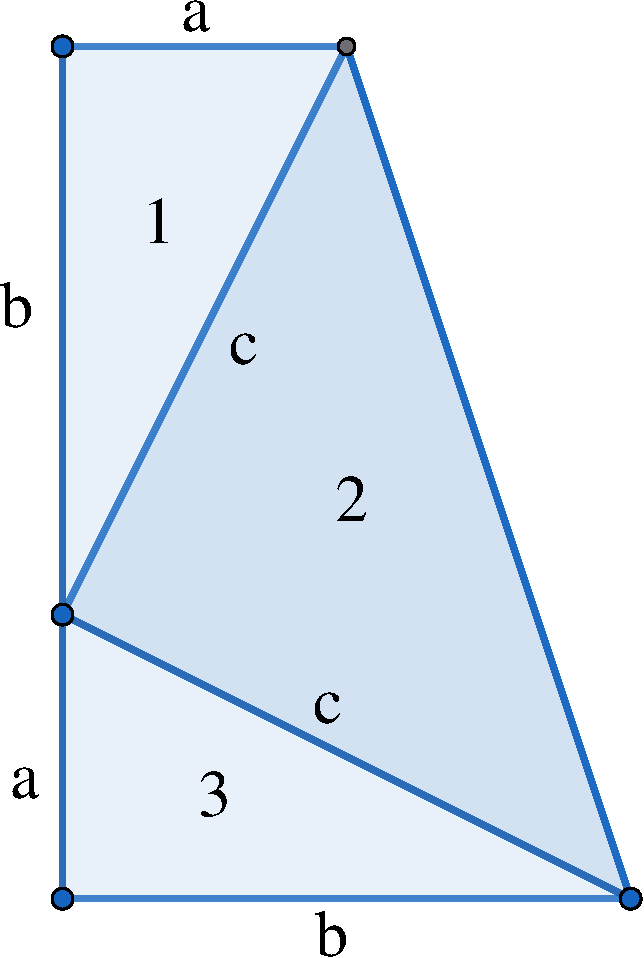
\includegraphics[scale=0.3]{img/garfield}
 \captionof{figure}{美国总统詹姆斯·加菲尔德证法(1876)}
 \label{fig:garfield}
\end{center}
}
\Question{$a, b$是互素的奇数,证明$\frac{a \pm b}{2}$互素。\label{qn:coprime-of-half-a-pm-b}}
\Question{$a, b$互素,若$ab = c^2$证明$a, b$都是平方数。\label{qn:coprime-product-as-square}}
\Question{利用埃拉托斯特尼筛法找出100以内的所有素数。\label{qn:seive-of-eratosthenes-100}}
\end{Exercise}

\begin{Answer}[ref={ex:irrationals}]
\Question{正五边形数}
\Question{梯形面积等于两个原直角三角形和一个等腰直角三角形的面积和
}
\Question{%%$a, b$是互素的奇数,证明$\frac{a \pm b}{2}$互素。
  \begin{proof}
    设$d$为$\frac{a \pm b}{2}$的公因子,令$dm = \frac{a + b}{2}, dn = \frac{a - b}{2}$,其中$m, n$为整数。两式相加求得$a = dm + dn = d(m + n)$,所以$d$整除$a$;两式相减得$b = dm - dn = d (m - n)$,所以$d$也整除$b$。这样$d$也是$a, b$的公因子。但$a, b$互素,所以$d$只能是1,即$\frac{a \pm b}{2}$互素。
  \end{proof}
}
\Question{%%$a, b$互素,若$ab = c^2$证明$a, b$都是平方数。
  \begin{proof}
    把$a, b$各自表示为素数幂的积:$a = p_1^{a_1} p_2^{a_2} \dotsm p_n^{a_n}, b = q_1^{b_1} q_2^{b_2} \dotsm q_m^{b_m}$,其中$p_i, q_j$都是素数。由于$a, b$互素,它们没有任何不等于1的公因数,故$p_i \ne q_j$。它们的积是个平方数$c^2 = p_1^{a_1} p_2^{a_2} \dotsm p_n^{a_n} q_1^{b_1} q_2^{b_2} \dotsm q_m^{b_m}$,所以必然有$a_i, b_j$全部是偶数,即$a, b$都是平方数。
  \end{proof}
}

\Question{%%利用埃拉托斯特尼筛法找出100以内的所有素数。
}
\end{Answer}

\ifx\wholebook\relax \else
\section{参考答案}
\shipoutAnswer

\subimport{inc/}{evenpfnum-zh-cn}

\begin{thebibliography}{99}
\subimport{inc/}{bib-zh-cn}
\end{thebibliography}

\expandafter\enddocument
\fi
